% Datasheet skAInet Edge-Compute v1.5 (Chinese, Simplified)
\documentclass[10pt,a4paper]{article}
\usepackage[margin=20mm,top=18mm,bottom=20mm]{geometry}
\usepackage{fontspec}
\usepackage{xeCJK}
\setmainfont{DejaVu Sans}
\setsansfont{DejaVu Sans}
\renewcommand{\familydefault}{\sfdefault}
\setCJKmainfont{Noto Sans CJK SC}
\setCJKsansfont{Noto Sans CJK SC}
\usepackage{booktabs,array,tabularx,siunitx,microtype}
\usepackage{tikz}
\usetikzlibrary{calc,arrows.meta}
\usepackage{xcolor}
\usepackage{graphicx}
\definecolor{skred}{HTML}{C8102E}
\definecolor{skgray}{HTML}{444444}
\usepackage{fancyhdr}
\pagestyle{fancy}\fancyhf{}
\fancyhead[L]{\small\textbf{skAInet Edge-Compute v1.5} — 产品数据手册}
\fancyhead[R]{\small Auto-Intern GmbH · 德国波鸿}
\fancyfoot[L]{\small DS-EC-1.5 · 2026 年 9 月}
\fancyfoot[R]{\small 第 \thepage 页}
\renewcommand{\headrulewidth}{0.4pt}
\setlength{\parindent}{0pt}
\sisetup{per-mode=symbol}

% dimensioning styles
\tikzset{
  dimline/.style={<->, >=Latex, line width=0.4pt, draw=skgray},
  extline/.style={line width=0.3pt, draw=skgray},
  dimtext/.style={fill=white, inner sep=1pt, font=\footnotesize, text=black},
  part/.style={line width=0.8pt, draw=black},
  hidden/.style={line width=0.4pt, draw=skgray, dash pattern=on 2pt off 1.5pt},
  center/.style={line width=0.3pt, draw=skgray, dash pattern=on 6pt off 1.5pt on 1pt off 1.5pt},
}

\begin{document}

%=====================================================================
% Page 1 — Overview & specification
%=====================================================================
\begin{minipage}[b]{0.66\textwidth}
{\LARGE\textbf{\textcolor{skred}{skAInet} Edge-Compute}}\quad{\Large v1.5}

\vspace{2mm}
{\large 可编程 M12-PoE 交换机、路由器与 Linux 计算模块，面向工业边缘数据采集}
\end{minipage}\hfill
\begin{minipage}[b]{0.26\textwidth}
\raggedleft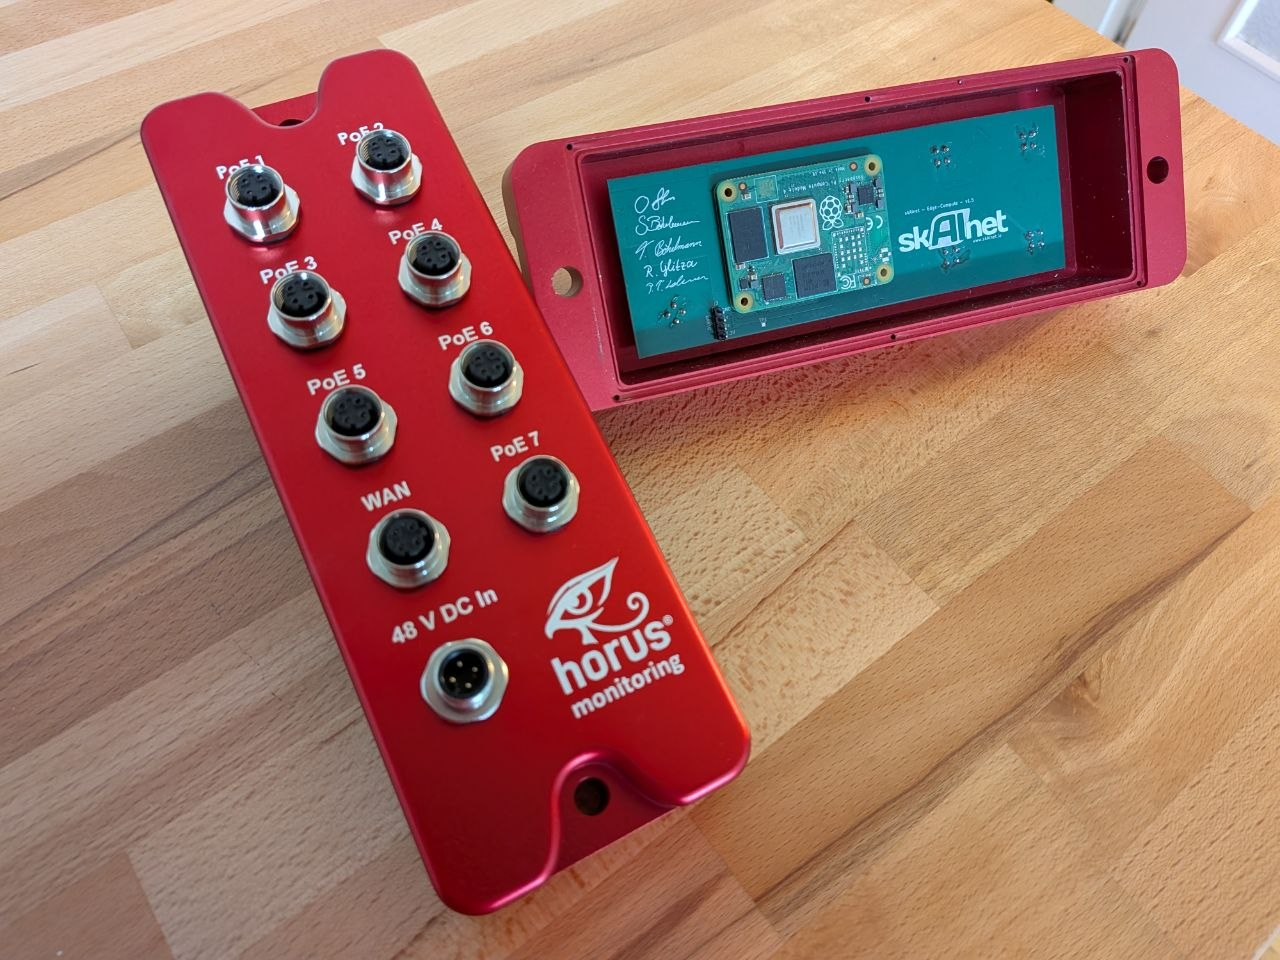
\includegraphics[width=\textwidth]{edge-branded.jpg}
\end{minipage}

\vspace{2mm}\hrule\vspace{2mm}

\textbf{产品简介。} skAInet Edge-Compute 是 Auto-Intern GmbH 的通用数据采集与监测平台。整块铣削的阳极氧化铝外壳集成了一个 8 口交换机（其中 7 个外部 M12 PoE+ LAN 端口，D 编码）、一个独立的 M12 WAN 端口（D 编码）以及可更换的计算模块（与 Raspberry Pi CM 引脚兼容）。所有接口均采用密封 M12 连接器；设备可在最深 \SI{1}{bar} 水压下工作。测量数据在设备上缓存、预处理和分析；只有明确配置转发的数据才会进入上游网络。

\vspace{2mm}
\begin{minipage}[t]{0.48\textwidth}
\textbf{计算}\par\vspace{1mm}
\begin{tabularx}{\textwidth}{@{}>{\bfseries}p{2.9cm}X@{}}
\toprule
模块 & Raspberry Pi CM4（标准）；可选 CM5 或 NVIDIA Jetson，引脚兼容、可更换 \\
CPU & 8 核 64 位 ARM，\SI{1.5}{GHz} \\
内存 & \SI{8}{GB} LPDDR4-3200 \\
存储 & \SI{32}{GB} eMMC \\
操作系统 & Yocto Linux，附完整 SBOM（符合欧盟《网络弹性法案》）；加密 OTA 更新或通过 USB 镜像离线更新 \\
\bottomrule
\end{tabularx}

\vspace{2mm}
\textbf{网络}\par\vspace{1mm}
\begin{tabularx}{\textwidth}{@{}>{\bfseries}p{2.9cm}X@{}}
\toprule
WAN & 1$\times$ M12 D 编码（4 芯），千兆以太网，DHCP 客户端 \\
LAN & 7$\times$ M12 D 编码（4 芯以太网）带 PoE+，内部接入 8 口交换机（DHCP 服务器，192.168.199.1/24）\\
PoE & 全部 7 个 LAN 端口支持 IEEE~802.3at（PoE+）；典型设备功耗约 \SI{10}{W} \\
布线 & 每台设备一根经认证的 Cat-5e M12 线缆 \\
数据接口 & 实时数据通过 WebSocket（端口 8001，JSON，纳秒时间戳）\\
上游 API & REST、WebSocket、Webhooks、MQTT、OPC~UA、Modbus-TCP、EPICS、gRPC、AMQP、CoAP、SNMP、Prometheus、InfluxDB、SFTP/rsync \\
容量 & 250+ 并发通道已在生产环境验证 \\
\bottomrule
\end{tabularx}
\end{minipage}\hfill
\begin{minipage}[t]{0.48\textwidth}
\textbf{供电}\par\vspace{1mm}
\begin{tabularx}{\textwidth}{@{}>{\bfseries}p{2.9cm}X@{}}
\toprule
输入 & \SIrange{48}{72}{V} DC，经 M12 A 编码（4 芯，TE T4140012041-000）\\
电源 & 建议 $\geq$ \SI{100}{W} \\
最低 & \SI{25}{W}（仅计算模块，无 PoE 负载）\\
\bottomrule
\end{tabularx}

\vspace{2mm}
\textbf{环境与机械}\par\vspace{1mm}
\begin{tabularx}{\textwidth}{@{}>{\bfseries}p{2.9cm}X@{}}
\toprule
外壳 & 阳极氧化铝，整块铣削，抗冲击 \\
防护等级 & IP67，所有端口和背板密封；可在最深 \SI{1}{bar} 水压下工作 \\
工作温度 & \SIrange{-25}{70}{\celsius} \\
外形尺寸 & $216 \times 75 \times 32$ \si{mm}（宽$\times$深$\times$高）；含连接器总深约 \SI{51}{mm} \\
面板 & 8$\times$ M12 D 编码（7$\times$ PoE LAN，1$\times$ WAN），4$\times$2 阵列；1$\times$ M12 A 编码电源输入；可定制品牌标识 \\
\bottomrule
\end{tabularx}

\vspace{2mm}
\textbf{软件}\par\vspace{1mm}
\begin{tabularx}{\textwidth}{@{}>{\bfseries}p{2.9cm}X@{}}
\toprule
访问 & SSH（端口 22022）；可用 C++ 或 Python 编写应用，Docker 部署；GitHub 提供最小示例 \\
远程维护 & 可选的厂商加密远程维护，可随时关闭 \\
更新 & 通过 WAN 端口加密 OTA 更新，或通过 USB 镜像离线更新 \\
\bottomrule
\end{tabularx}

\vspace{2mm}
\textbf{现场应用案例}\par\vspace{1mm}
{\small DB Netz DIANA（道岔电机监测）· Kelvion（红外污垢检测）· Kurtz Ersa / Global Point HORUS（焊接过程监测）· RUB/GSI-FAIR PANDA（亮度探测器）· MSU CBE（河流阻抗谱）· NexuFed AI / RUB（联邦学习泵监测）}
\end{minipage}

\vspace{2mm}\hrule\vspace{1.5mm}
{\small
\textbf{制造商：} Auto-Intern GmbH · Herner Str.\ 299, Geb.\ B29, 44809 Bochum, 德国 · info@auto-intern.de · +49\,234\,9345\,1121\\
\textbf{价格：} 260\,欧元 / 299\,美元（净价）起 · \textbf{文档：} edge-compute.skainet.io}

%=====================================================================
% Sheets 1-3 — dimensioned drawing 1:1, one view per page, module vertical
%=====================================================================
\newpage
\thispagestyle{fancy}
\begin{center}
{\large\textbf{尺寸图 — Edge-Compute v1.5 外壳}}\\[1mm]
{\small 所有尺寸单位为 mm · 一般公差 ISO 2768-mK · 材料：铝，阳极氧化 · \textbf{比例 1:1} · 图纸 1/4：正视图}
\end{center}
\vfill
\begin{center}
\begin{tikzpicture}[scale=0.1, rotate=90]  % 1:1, module vertical
  % outer contour 216 x 75, corner radius 10
  \draw[part, rounded corners=1cm] (-108,-37.5) rectangle (108,37.5);
  \draw[center] (-114,0) -- (114,0);
  \draw[center] (0,-43) -- (0,43);
  % M12 sockets D-coded, 4x2 grid, pitch 32/32
  \foreach \x in {-64,-32,0,32}{
    \foreach \y in {-16,16}{
      \begin{scope}[shift={(\x,\y)}]
        \draw[part] (6.75,{sqrt(64-6.75*6.75)}) arc[start angle={acos(6.75/8)}, end angle={180-acos(6.75/8)}, radius=8];
        \draw[part] (-6.75,{-sqrt(64-6.75*6.75)}) arc[start angle={180+acos(6.75/8)}, end angle={360-acos(6.75/8)}, radius=8];
        \draw[part] (6.75,{sqrt(64-6.75*6.75)}) -- (6.75,{-sqrt(64-6.75*6.75)});
        \draw[part] (-6.75,{sqrt(64-6.75*6.75)}) -- (-6.75,{-sqrt(64-6.75*6.75)});
        \draw[part] (0,0) circle[radius=6];
        \draw[part] (0,0) circle[radius=4.5];
        \foreach \a in {45,135,225,315} \fill (\a:2.6) circle[radius=0.6];
        \draw[center] (-10,0)--(10,0); \draw[center] (0,-10)--(0,10);
      \end{scope}
    }
  }
  % power socket A-coded, rotated 45°
  \begin{scope}[shift={(64,-16)}, rotate=45]
    \draw[part] (6.75,{sqrt(64-6.75*6.75)}) arc[start angle={acos(6.75/8)}, end angle={180-acos(6.75/8)}, radius=8];
    \draw[part] (-6.75,{-sqrt(64-6.75*6.75)}) arc[start angle={180+acos(6.75/8)}, end angle={360-acos(6.75/8)}, radius=8];
    \draw[part] (6.75,{sqrt(64-6.75*6.75)}) -- (6.75,{-sqrt(64-6.75*6.75)});
    \draw[part] (-6.75,{sqrt(64-6.75*6.75)}) -- (-6.75,{-sqrt(64-6.75*6.75)});
    \draw[part] (0,0) circle[radius=6];
    \draw[part] (0,0) circle[radius=4.5];
    \foreach \a in {45,135,225,315} \fill (\a:2.6) circle[radius=0.6];
    \draw[center] (-10,0)--(10,0); \draw[center] (0,-10)--(0,10);
  \end{scope}
  \node[font=\scriptsize, text=skgray, anchor=west] at (64,-40) {电源输入（M12 A 编码，4 芯），45°};
  % dimension 216 (vertical after rotation)
  \draw[extline] (-108,37.5) -- (-108,48);
  \draw[extline] (108,37.5) -- (108,48);
  \draw[dimline] (-108,45) -- (108,45) node[dimtext,midway,rotate=90]{216};
  % dimension 75 (horizontal after rotation)
  \draw[extline] (-108,-37.5) -- (-119,-37.5);
  \draw[extline] (-108,37.5) -- (-119,37.5);
  \draw[dimline] (-116,-37.5) -- (-116,37.5) node[dimtext,midway]{75};
  % grid pitch 32
  \draw[extline] (-64,-16) -- (-64,-48);
  \draw[extline] (-32,-16) -- (-32,-48);
  \draw[dimline] (-64,-45) -- (-32,-45) node[dimtext,midway,rotate=90]{32};
  \draw[extline] (0,16) -- (0,52);
  \draw[extline] (32,16) -- (32,52);
  \draw[dimline] (0,49) -- (32,49) node[dimtext,midway,rotate=90]{32 (4$\times$)};
  \draw[extline] (-64,16) -- (-86,16);
  \draw[extline] (-64,-16) -- (-86,-16);
  \draw[dimline] (-83,-16) -- (-83,16) node[dimtext,midway]{32};
  % labels
  \node[dimtext, anchor=west] at (-95,44) {8$\times$ M12 D 编码（以太网，4 芯）};
  \draw[extline] (-88,42) -- (-70,18);
  \node[dimtext] at (100,25) {R10 (4$\times$)};
  % 2x Ø8.5 mounting holes in the lugs (at ±98, centered)
  \foreach \x in {-98,98}{
    \draw[part] (\x,0) circle[radius=4.25];
    \draw[center] (\x-8,0)--(\x+8,0); \draw[center] (\x,-8)--(\x,8);
  }
  \draw[extline] (-98,0) -- (-98,-55);
  \draw[extline] (98,0) -- (98,-55);
  \draw[dimline] (-98,-52) -- (98,-52) node[dimtext,midway,rotate=90]{196};
  \node[dimtext, anchor=east] at (93,-14) {2$\times$ Ø8.5（安装孔）};
  \node[font=\small\bfseries, rotate=90] at (0,-62) {正视图 — 连接器侧};
\end{tikzpicture}
\end{center}
\vfill

\newpage
\thispagestyle{fancy}
\begin{center}
{\small 所有尺寸单位为 mm · \textbf{比例 1:1} · 图纸 2/4：底视图}
\end{center}
\vfill
\begin{center}
\begin{tikzpicture}[scale=0.1, rotate=90]
  \draw[part, rounded corners=1cm] (-108,-37.5) rectangle (108,37.5);
  \draw[center] (-114,0) -- (114,0);
  \draw[center] (0,-43) -- (0,43);
  % pocket 166x58 R3 t30
  \draw[hidden, rounded corners=0.3cm] (-83,-29) rectangle (83,29);
  % 6x M3x30 cover screws
  \foreach \x in {-70,0,70}{
    \foreach \y in {-25,25}{
      \draw[part] (\x,\y) circle[radius=1.5];
      \draw[center] (\x-4,\y)--(\x+4,\y); \draw[center] (\x,\y-4)--(\x,\y+4);
    }
  }
  % dimensions
  \draw[extline] (-83,-29) -- (-83,-50);
  \draw[extline] (83,-29) -- (83,-50);
  \draw[dimline] (-83,-47) -- (83,-47) node[dimtext,midway,rotate=90]{166（凹腔，深 30，R3）};
  \draw[extline] (-83,29) -- (-119,29);
  \draw[extline] (-83,-29) -- (-119,-29);
  \draw[dimline] (-116,-29) -- (-116,29) node[dimtext,midway]{58};
  \draw[extline] (-108,37.5) -- (-108,48);
  \draw[extline] (108,37.5) -- (108,48);
  \draw[dimline] (-108,45) -- (108,45) node[dimtext,midway,rotate=90]{216};
  \node[dimtext, anchor=west] at (-60,-38) {6$\times$ M3$\times$30（盖板螺钉）};
  \draw[extline] (-55,-36) -- (-68.5,-26.5);
  \node[font=\small\bfseries, rotate=90] at (0,-60) {底视图 — 凹腔与盖板螺钉};
\end{tikzpicture}
\end{center}
\vfill

\newpage
\thispagestyle{fancy}
\begin{center}
{\small 所有尺寸单位为 mm · \textbf{比例 1:1} · 图纸 3/4：侧视图}
\end{center}
\begin{center}
\begin{tikzpicture}[scale=0.1, rotate=90]
  % profile: base 20 + cover 12 = 32
  \draw[part] (-108,0) -- (108,0) -- (108,32) -- (-108,32) -- cycle;
  \draw[hidden] (-108,20) -- (108,20);
  % M12 connectors (protrusion 19: hex, threaded body, coupling ring)
  \foreach \x in {-64,-32,0,32,64}{
    \draw[part] (\x-9,32) -- (\x-9,36) -- (\x-7.5,36) -- (\x-7.5,44)
      -- (\x-8,44) -- (\x-8,51) -- (\x+8,51) -- (\x+8,44)
      -- (\x+7.5,44) -- (\x+7.5,36) -- (\x+9,36) -- (\x+9,32);
    \draw[center] (\x,30) -- (\x,54);
  }
  \node[dimtext, rotate=90, anchor=west] at (80,56) {M12（9$\times$）};
  % height dimensions
  \draw[extline] (108,0) -- (117,0);
  \draw[extline] (108,20) -- (117,20);
  \draw[extline] (108,32) -- (117,32);
  \draw[extline] (88,51) -- (117,51);
  \draw[dimline] (114,0) -- (114,20) node[dimtext,midway]{20};
  \draw[dimline] (114,20) -- (114,32) node[dimtext,midway]{12};
  \draw[dimline] (114,32) -- (114,51) node[dimtext,midway]{19};
  \draw[extline] (-108,0) -- (-117,0);
  \draw[extline] (-108,32) -- (-117,32);
  \draw[dimline] (-114,0) -- (-114,32) node[dimtext,midway]{32};
  \draw[extline] (-108,0) -- (-108,-9);
  \draw[extline] (108,0) -- (108,-9);
  \draw[dimline] (-108,-6) -- (108,-6) node[dimtext,midway,rotate=90]{216};
  \node[dimtext, rotate=90] at (30,16) {盖板轮廓带握槽，边缘圆角 R3};
  \node[font=\small\bfseries, rotate=90] at (0,-18) {侧视图};
\end{tikzpicture}
\end{center}

\newpage
\thispagestyle{fancy}
\begin{center}
{\small 图纸 4/4：计算模块等轴测图，连接器侧（非比例）}
\end{center}
\vfill
\begin{center}
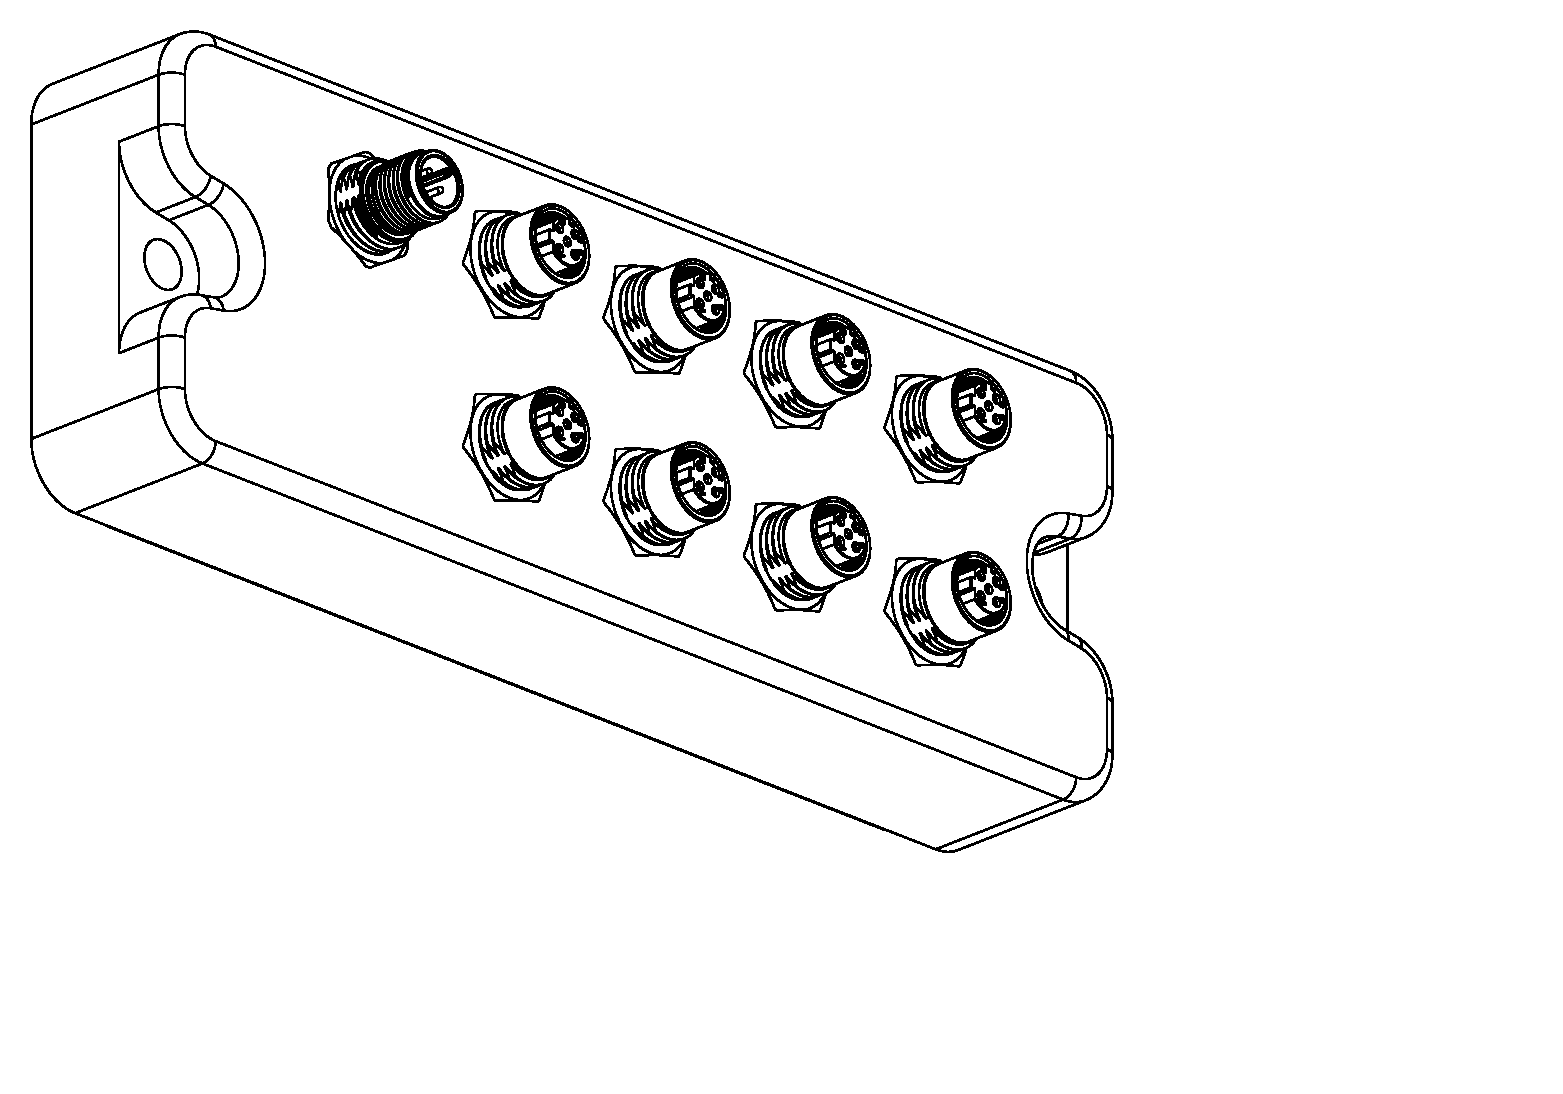
\includegraphics[width=0.95\textwidth]{horus-assembly.pdf}
\end{center}
\vfill
{\scriptsize 所有连接器均为 M12、IP67：8$\times$ D 编码（7$\times$ PoE LAN，1$\times$ WAN，4 芯以太网），间距 $32\times32$；1$\times$ A 编码电源输入（4 芯），旋转 45°。盖板紧固：6$\times$ M3$\times$30。规格如有变更，恕不另行通知。}

\end{document}
